\documentclass[border=1pt]{standalone}
\usepackage{newtxtext,newtxmath}
\usepackage{pgfplots}
\usetikzlibrary{calc}
\pgfplotsset{compat=1.18}
\definecolor{obs}{HTML}{D55E00}
\definecolor{sens}{HTML}{0072B2}
\begin{document}
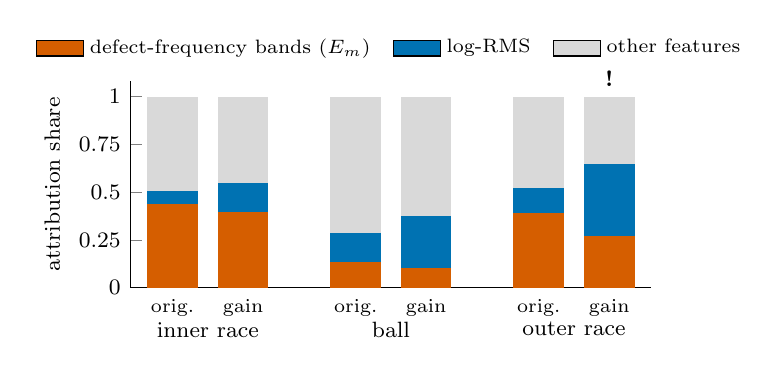
\begin{tikzpicture}
\begin{axis}[width=8.2cm, height=4.2cm, xmin=-0.6, xmax=6.8, ymin=0, ymax=1.08,
  axis x line*=bottom, axis y line*=left, clip=false, xtick={0.5,3.1,5.7},
  xticklabels={inner race,ball,outer race}, xticklabel style={font=\footnotesize, yshift=-9pt},
  x tick style={draw=none}, ytick={0,0.25,0.5,0.75,1}, yticklabel style={font=\footnotesize, /pgf/number format/fixed},
  ylabel={attribution share}, ylabel style={font=\footnotesize},
  legend style={draw=none, fill=none, font=\scriptsize, at={(0.5,1.06)}, anchor=south, legend columns=3,
    /tikz/every even column/.append style={column sep=6pt}}, legend cell align=left]
\addlegendimage{area legend, fill=obs, draw=none}\addlegendentry{defect-frequency bands ($E_m$)}
\addlegendimage{area legend, fill=sens, draw=none}\addlegendentry{log-RMS}
\addlegendimage{area legend, fill=black!15, draw=none}\addlegendentry{other features}
\fill[obs] (axis cs:-0.36,0) rectangle (axis cs:0.36,0.4404);
\fill[sens] (axis cs:-0.36,0.4404) rectangle (axis cs:0.36,0.5083);
\fill[black!15] (axis cs:-0.36,0.5083) rectangle (axis cs:0.36,1);
\node[font=\scriptsize, anchor=north] at (axis cs:0.0,-0.01) {orig.};
\fill[obs] (axis cs:0.64,0) rectangle (axis cs:1.3599999999999999,0.3937);
\fill[sens] (axis cs:0.64,0.3937) rectangle (axis cs:1.3599999999999999,0.5503);
\fill[black!15] (axis cs:0.64,0.5503) rectangle (axis cs:1.3599999999999999,1);
\node[font=\scriptsize, anchor=north] at (axis cs:1.0,-0.01) {gain};
\fill[obs] (axis cs:2.24,0) rectangle (axis cs:2.96,0.1331);
\fill[sens] (axis cs:2.24,0.1331) rectangle (axis cs:2.96,0.2836);
\fill[black!15] (axis cs:2.24,0.2836) rectangle (axis cs:2.96,1);
\node[font=\scriptsize, anchor=north] at (axis cs:2.6,-0.01) {orig.};
\fill[obs] (axis cs:3.24,0) rectangle (axis cs:3.96,0.1047);
\fill[sens] (axis cs:3.24,0.1047) rectangle (axis cs:3.96,0.3752);
\fill[black!15] (axis cs:3.24,0.3752) rectangle (axis cs:3.96,1);
\node[font=\scriptsize, anchor=north] at (axis cs:3.6,-0.01) {gain};
\fill[obs] (axis cs:4.839999999999999,0) rectangle (axis cs:5.56,0.3922);
\fill[sens] (axis cs:4.839999999999999,0.3922) rectangle (axis cs:5.56,0.5191);
\fill[black!15] (axis cs:4.839999999999999,0.5191) rectangle (axis cs:5.56,1);
\node[font=\scriptsize, anchor=north] at (axis cs:5.199999999999999,-0.01) {orig.};
\fill[obs] (axis cs:5.839999999999999,0) rectangle (axis cs:6.56,0.2694);
\fill[sens] (axis cs:5.839999999999999,0.2694) rectangle (axis cs:6.56,0.6489);
\fill[black!15] (axis cs:5.839999999999999,0.6489) rectangle (axis cs:6.56,1);
\node[font=\scriptsize, anchor=north] at (axis cs:6.199999999999999,-0.01) {gain};
\node[font=\footnotesize\bfseries, anchor=south] at (axis cs:6.199999999999999,1.0) {!};
\end{axis}
\end{tikzpicture}
\end{document}
